The Simplified Pushover-based Earthquake Loss Assessment methodology \citep{BorziEtAl2008b} allows the calculation of the displacement capacity (i.e. spectral displacement) and collapse multiplier (i.e. spectral acceleration) using a mechanics-based procedure, similar to what has been proposed by \citet{CosenzaEtAl2005}. The methodology implemented in the Risk Modeller's Toolkit currently only uses the displacement capacity equations of SP-BELA for reinforced concrete frames (and does not yet estimate the collapse multiplier using the simplified pushover approach of SP-BELA). The full SP-BELA methodology will be implemented in the future, together with the similar process that has also been proposed for masonry structures \citep{BorziEtAl2008a}.\\

The original methodology as proposed by \citet{BorziEtAl2008b} considered three limit states (light damage corresponding to the yielding point, significant damage, and collapse). However, other limit states can be considered, granted that the user provides the information required to establish each limit state.\\

The spectral displacement at each limit state is calculated by firstly assessing the expected chord rotation at the associated damage threshold, and then multiplying this rotation by the height of the equivalent single degree of freedom (SDoF) system. The rotation at the yielding point ($\Theta_y$)can be calculated using the formula below, as proposed by \citet{CosenzaEtAl2005} and \citet{PanagiotakosFardis2001}:

\begin{equation}
	\Theta_y = \phi_y\frac{L_V}{3}+0.0013\left(1 + 1.5\frac{h}{L_V}\right)+0.13\phi_y\frac{d_bf_y}{\sqrt{f_c}}
\end{equation}

Where $\phi_y$ stands for the yield curvature of the section, $L_V$ represents the shear span (which for columns can be assumed as half of the inter-storey height \citep{BorziEtAl2008b}), $h$ stands for the section height, $d_b$ is the longitudinal bar diameter, and $f_y$ and $f_c$ are the strength of the steel and concrete (in MPa), respectively. The yield curvature ($\phi_y$) can be calculated using the equation proposed by \cite{PriestleyEtAl2007}:

\begin{equation}
	\phi_y = 2.14\frac{\epsilon_y}{h}
\end{equation}

Where $\epsilon_y$ represents the yield strain of the longitudinal rebars.\\

For what concerns the ultimate rotation capacity ($\Theta_u$), \cite{PanagiotakosFardis2001} proposed the following formula:

\begin{equation}
	\Theta_u = \frac{1}{\gamma_{el}}\left[\Theta_y + (\phi_u-\phi_y)L_{pl}\left(1-\frac{0.5L_pl}{L_V}\right)\right]
\end{equation}

Where $\gamma_{el}$ is 1.5 for the primary structural elements and 1 for all others \citep{BorziEtAl2008b}, $\phi_u$ stands for the ultimate curvature, and $L_pl$ is the plastic hinge length, which can be computed through the following equation:

\begin{equation}
	\phi_u = \frac{\epsilon_{cu}+\epsilon_{su}}{h}
\end{equation}

Where $\epsilon_{cu}$ and $\epsilon_{su}$ are the ultimate concrete and steel strain, respectively. These two parameters depend on the level of confinement of the reinforced concrete and expected ductility, and reasonable ranges can be found in \cite{Calvi1999}, \cite{CrowleyEtAl2004} or \cite{BalEtAl2010}.\\

Other rotation thresholds (corresponding to other limit states) can also be calculated, either through the definition of concrete and steel strains (e.g. \cite{CrowleyEtAl2004}), or as a fraction of the previously described rotations. For example, \cite{BorziEtAl2008b} defined the limit state for significant damage as $^3/_4$ of the ultimate rotation capacity ($\Theta_u$).\\

As previously mentioned, the spectral displacement at each limit state can be calculated by multiplying the respective rotation by the height of the equivalent SDoF system. This height is calculated by multiplying the total height of the structure ($H_T$) by an effective height ratio ($ef_h$). The calculation of this ratio depends on the expected failure mechanism (beam sway or column sway - see Figure~\ref{fig:mechanisms}), and its calculation has been explained in Section~\ref{subsec:DBELA}. For the yielding point, the spectral displacement can then be calculated as follows:

\begin{equation}
	\Delta_y = \Theta_yef_hH_T
\end{equation}

The displacement capacity at the remaining limit states depends on the expected failure mechanisms (as defined in Figure~\ref{fig:mechanisms}), and can be calculated using the following formulae:\\

For beam sway:

\begin{equation}
	\Delta_{LS_i} = \Delta_y + (\Theta_{LS_i} - \Theta_y)ef_hH_T
\end{equation}

for column sway:
\begin{equation}
	\Delta_{LS_i} = \Delta_y + (\Theta_{LS_i} - \Theta_y)h_p
\end{equation}

Where $h_p$ stands for the ground storey height.

The calculation of the spectral aceleration for each limit states follows the same procedure explained in the previous Section, in which an elasto-plastic behaviour is assumed, and the following formula is employed to calculate acceleration at the yielding point:

\begin{equation}
	Sa_i = \frac{4\pi^2Sd_i}{T_y^2}
\end{equation}

Where $T_y$ stands for the yielding period which is currently calculated using simplified formulae (e.g. \cite{CrowleyPinho2004}; \cite{CrowleyPinho2006}), as further explained in Section \ref{subsec:DBELA_Silva2013}, rather than based on estimating the collapse multiplier as in the original SP-BELA methodology.\\

To use this methodology it is necessary to define a building model, which specifies the probabilistic distribution of the geometrical and material properties. This information is currently stored in a $csv$ file (tabular format), as presented in Table \ref{table:building_model}.

\begin {table}[htb]
\caption{Example of a building model compatible with the SPBELA method}
\label{table:building_model}
\begin{center}
  \begin{tabular}{ | l | l | l | l | l | l |}
  \hline
Structure type & bare frame &  &  &  &  \\ \hline
ductility & ductile &  &  &  &  \\ \hline
number of storeys & 3 &  &  &  &  \\ \hline
steel modulus & lognormal & 210000 & 0.01 & 0 & $\infty$ \\ \hline
concrete strength & normal & 30 & 0.05 & 0 & $\infty$ \\ \hline
steel bar diameter & discrete & 0.01 & 1 & 0 & $\infty$ \\ \hline
steel yield strength & normal & 371.33 & 0.24 & 0 & $\infty$ \\ \hline
ground floor height & discrete & 2.8 3.1 3.2 & 0.48 0.15 0.37 & 0 & $\infty$ \\ \hline
regular floor height & lognormal & 2.84 & 0.08 & 0 & $\infty$ \\ \hline
column depth & lognormal & 0.45 & 0.12 & 0.3 & 0.6 \\ \hline
beam length & gamma & 3.37 & 0.38 & 0 & $\infty$ \\ \hline
beam depth & lognormal & 0.6 & 0.16 & 0.4 & 0.8 \\ \hline
  \end{tabular}
\end{center}
\end{table}

The definition of each parameter follows the same approach described in the previous Section for the Displacement-based Earthquake Loss Assessment (DBELA) methodology.

The location of the building model and the damage model (see Section \ref{subsec:dmg_model}) should be specified in the variables \verb=building_model= and the \verb=damage_model=, respectively. The number of capacity curves that should be generated must be defined using the parameter \verb=no_assets=. Then, after importing the module \verb=SPBELA=, the set of capacity curves can be generated using the following commands:

\begin{Verbatim}[frame=single, commandchars=\\\{\}, samepage=true]
building_class_model = SPBELA.read_building_class_model(building_model)
assets = SPBELA.generate_assets(building_class_model,no_assets)
capacity_curves = SPBELA.generate_capacity_curves(assets,damage_model)
\end{Verbatim}

The first function (\verb=read_building_class_model=) processes the information about the building class; the second function (\verb=generate_assets=) uses a Monte Carlo sampling process to generate a set of synthetic structural models (each one with unique geometrical and material properties); and the final function (\verb=generate_capacity_curves=) combines the generated assets with the damage model to calculate a capacity curve per structure. Figure \ref{fig:SPBELA_cc} presents a collection of capacity curves generated using this methodology.

\begin{figure}[htb]
  \centering
      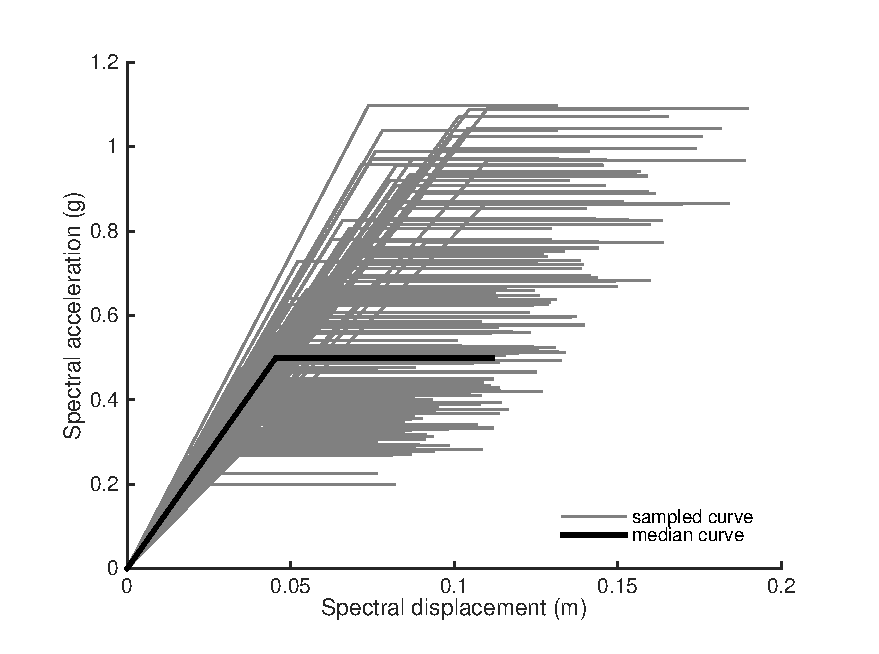
\includegraphics[width=8cm]{Figures/SPBELA_cc.eps}
  \caption{Capacity curves for reinforced concrete bare frames generated using the SPBELA methodology.}
  \label{fig:SPBELA_cc}
\end{figure}